\begin{document}
\maketitle

\begin{abstract}
We build a fall detector for the Pepper robot that fuses ST-GCN skeleton motion with a frozen Qwen2.5-VL.
All models we train on FallVision reach a video AUROC of 0.99, but a classifier on a \emph{single} skeleton frame already reaches 0.942: the models detect a lying posture, not a fall.
Training on segment-level fall labels makes ST-GCN rely on motion and raises AUROC on unseen datasets (GMDCSA24 0.932$\to$0.968).
No single modality is reliable on every unseen dataset; fusing both and training on 16 fall-related actions gives the most consistent model (mean unseen AUROC 0.911), although the fusion still uses skeleton motion only weakly.
\end{abstract}

\section{Introduction}

A home robot must notice when a person falls, and it must not raise an alarm when the person lies down on a bed or sits on the floor on purpose.
Both cases end in the same posture, so the detector has to use \emph{how} the person got there (motion) or \emph{where} they are (scene context).
A robot also sees people from a low, changing viewpoint, so a detector trained on fixed surveillance cameras must transfer to new views and new rooms.

Our proposal asked two questions.
\textbf{RQ1:} does explicit skeleton motion generalize better to unseen viewpoints than a VLM that reasons directly on RGB video?
\textbf{RQ2:} does semantic context from a VLM improve fall detection beyond skeleton motion alone?
For the midterm we first establish the baselines and answer both questions on datasets that the models never see during training, using the camera height of a synthetic dataset as a proxy for the robot view; evaluation on Pepper recordings builds on these baselines.
Our quantitative objectives are (i) AUROC on unseen datasets, (ii) the AUROC drop when motion is removed from the input, which tells whether a model uses motion at all, and (iii) the false-alarm rate on intentional lying and sitting.

So far we reproduce both baselines, show that the near-perfect in-domain scores come from a static-posture shortcut created by video-level labels, and test segment-level and 16-action labels and five fusion variants against it.

\section{Related Work}

\textbf{Skeleton-based fall detection.}
ST-GCN~\citep{yan2018stgcn} and its successors model joint trajectories as a spatio-temporal graph and report near-perfect accuracy on staged datasets.
Under a change of environment, skeleton models keep 71--81\% fall F1 while frozen RGB features drop to 0--49\%, and concatenating RGB features with the skeleton stream falls below the skeleton alone~\citep{lamsal2026safer}.
Yet a skeleton detector trained on a single staged dataset still collapses on another one (99\% on Le2i, $\sim$1\% fall F1 on NTU)~\citep{zobi2025vira}.
This suggests that the bottleneck is the training labels and data rather than the representation, which is what we test.

\textbf{VLM-based fall detection.}
Multimodal LLMs can detect falls zero-shot: on in-the-wild falls, Qwen3-VL and InternVL3.5 match fine-tuned video models, but on staged UP-Fall they label 95--97\% of \emph{fallen} clips as \emph{lying}~\citep{schneider2025omnifall}.
Video LLMs in general rely on single frames and are insensitive to frame order~\citep{liu2024tempcompass}.
Since a fall and a deliberate lie-down differ mainly in motion, this bias matters directly for our task; we measure it with reversed and frozen inputs.

\textbf{Datasets and robot-view detection.}
OmniFall~\citep{schneider2025omnifall} unifies staged, synthetic (OF-Syn), and in-the-wild data under a 16-class label set that separates the \emph{fall} event from the \emph{fallen} state and from intentional \emph{lie\_down}.
Robot systems mostly decide by geometry: a person is down if the upper body is within 0.7\,m of the estimated ground plane~\citep{solbach2017fallen}, verified from several viewpoints with a camera at 1.16\,m, close to Pepper's height~\citep{antonello2017fallen}.
To our knowledge, no fall detector has been published for Pepper.

\section{Method}

\subsection{Pipeline and models}
Figure~\ref{fig:pipeline} shows the pipeline.
Each video is cut into 1.6\,s clips (16 frames at 10\,fps, stride 8).
\textbf{Skeleton branch:} YOLO11x-pose~\citep{jocher2024yolo11} with ByteTrack~\citep{zhang2022bytetrack} gives 17 COCO joints; we keep the longest track.
Joints with confidence below 0.3 are masked.
We use two normalizations: \emph{Run A} keeps image coordinates in $[0,1]$, and \emph{Run B} centers on the hips and scales by torso length.
A 6-block ST-GCN (2.0M parameters) maps the $3\times16\times17$ input to a 256-d feature.
\textbf{VLM branch:} four frames of the same clip go to a frozen Qwen2.5-VL-7B~\citep{bai2025qwen25vl} with the prompt \emph{``Does any person fall down in this video? Answer with only Yes or No.''}
We read three outputs: $p_\mathrm{fall}=\sigma(\log\sum_\mathrm{Yes}e^{z}-\log\sum_\mathrm{No}e^{z})$ from the answer logits, the last-layer hidden state of the answer token (3584-d), and the video patch tokens pooled to a $2\times6\times6$ grid plus the answer token (73 tokens, \emph{tokmean} = their mean concatenated with the answer token).
\textbf{Fusion:} (a) \emph{concat}: LayerNorm and a linear projection to 128-d, concatenated with the ST-GCN feature, then a 2-layer MLP, with modality dropout 0.15; (b) \emph{cross-attention}: the $4\times17$ ST-GCN feature-map tokens attend to the 73 VLM tokens, with joint and patch positions in the same image coordinates.
A video score is the maximum over its clips.

\begin{figure}[t]
  \centering
  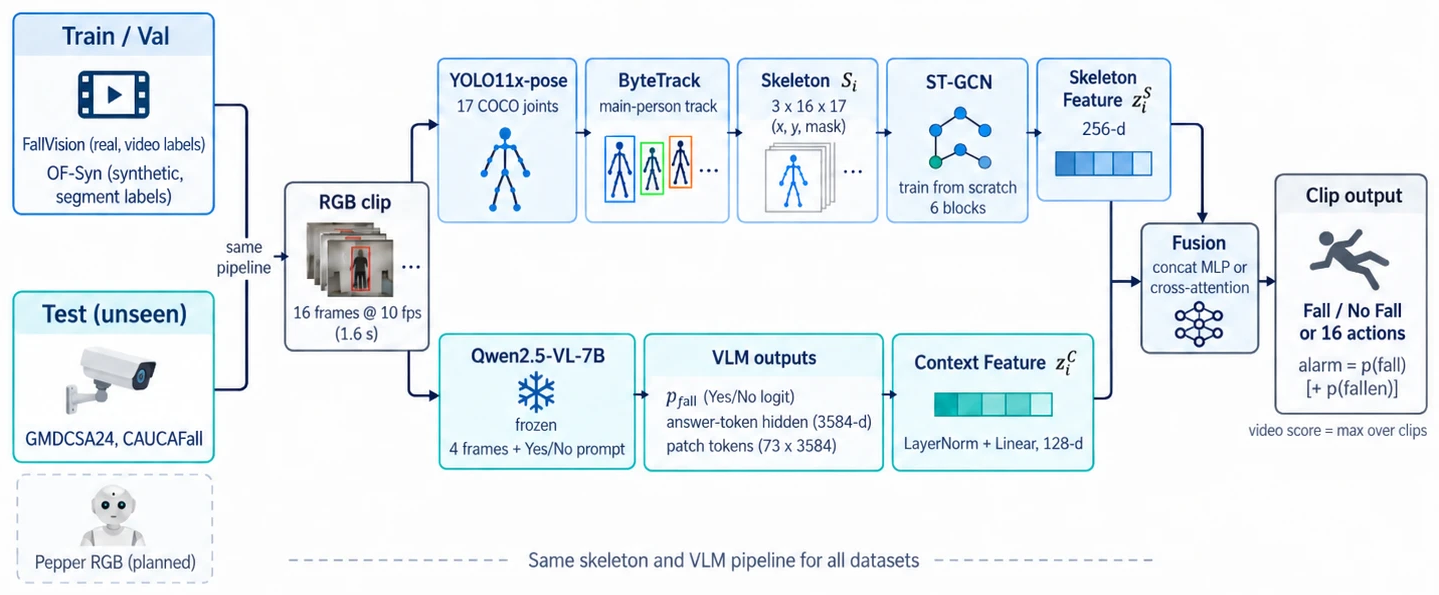
\includegraphics[width=\linewidth]{figs/pipeline.png}
  \caption{Pipeline. Both branches see the same 1.6\,s clip; the output is a binary fall score or a distribution over the 16 OmniFall actions.}
  \label{fig:pipeline}
\end{figure}

\subsection{Data and preprocessing}
Clips are 1.6\,s windows with stride 0.8\,s.
\textbf{FallVision}~\citep{rahman2025fallvision} has 5,866 videos with video-level labels and three scenarios (fall from bed, chair, standing).
We remove 262 exact or anonymized duplicates (md5) and split by recording session (perceptual-hash clusters of the background), so no room or take appears in two splits (15,569 / 1,841 / 1,660 train/val/test clips).
\textbf{OF-Syn}~\citep{schneider2025omnifall} has 12,000 synthetic videos with segment labels and camera-elevation metadata; we use the official split (57,600 / 7,200 / 7,200 clips) and transcode it from AV1 to H.264.
\textbf{GMDCSA24}~\citep{alam2024gmdcsa} and \textbf{CAUCAFall}~\citep{eraso2022caucafall} are used only for testing (160 and 100 videos, 1,512 and 1,188 clips), with the OmniFall segment labels.
We compare three clip labels:
\emph{video label} (every clip of a fall video is positive, as in FallVision);
\emph{event label} (positive if the clip overlaps a fall segment by $\geq$0.3\,s, negative if it does not overlap, ignored otherwise);
and the \emph{16 OmniFall actions} (the action that covers most of the clip).


\subsection{Metrics and loss}
Our main metric is \textbf{AUROC}, at the clip level (positive = overlaps a fall segment) and at the video level (positive = the video contains a fall).
We use AUROC rather than F1 because thresholds do not transfer across datasets (the FallVision threshold for recall 0.9 is 0.9956--0.99998 for the fusion models).
We add two diagnostics.
The \textbf{motion-removal test} repeats the last frame of each clip 16 times (for the VLM, four copies of the last frame); a model that uses motion should lose AUROC.
The \textbf{per-action alarm rate} is the fraction of clips of each OmniFall action scored above the threshold that gives recall 0.9 on OF-Syn validation.
Binary models are trained with class-weighted BCE ($w_+ = N_-/N_+$); the 16-action model uses cross-entropy with class weights $\propto n_c^{-1/2}$.
We use AdamW (lr $10^{-3}$, weight decay $10^{-4}$), a one-cycle schedule, batch 64, and flip, scale, rotation, and joint-drop augmentation; we report the mean of three seeds.

\subsection{Baselines}
\textbf{ST-GCN}~\citep{yan2018stgcn} is the standard skeleton action model and the skeleton-only configuration of our proposal.
\textbf{Zero-shot Qwen2.5-VL} is the RGB-only configuration: it needs no training, so it shows what a general VLM does on falls, and its $p_\mathrm{fall}$ is one of the fusion inputs.

\section{Experimental Results}

\subsection{Baseline reproduction}
Figure~\ref{fig:baseline} shows the confusion matrices on the FallVision test set (500 videos).
ST-GCN (Run A) reaches video AUROC $0.986\pm0.001$ and F1 $0.949\pm0.004$ at threshold 0.5 (validation AUROC saturates after about 20 of 50 epochs; logs in our repository).
Zero-shot Qwen2.5-VL reaches AUROC 0.941 and F1 0.806; most of its errors are missed falls (73 of 268).

\begin{table}[t]
  \makeatletter
  \begin{minipage}[c]{0.47\textwidth}
    \def\@captype{figure}
    \centering
    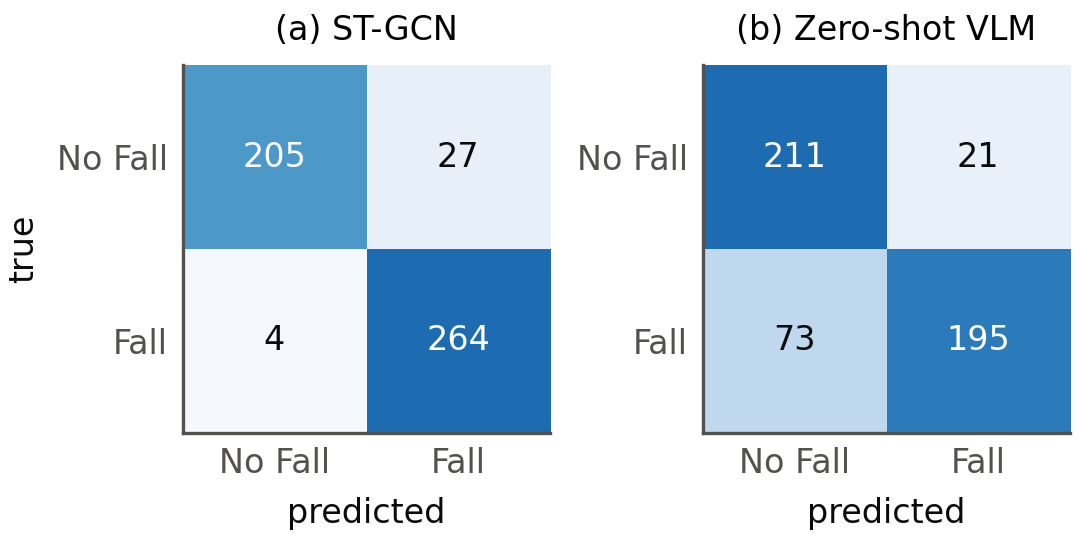
\includegraphics[width=\linewidth]{figs/baseline.png}
    \caption{FallVision test, video-level confusion matrices at threshold 0.5. (a) ST-GCN, Run A, seed 0. (b) Zero-shot Qwen2.5-VL.}
    \label{fig:baseline}
  \end{minipage}\hfill
  \begin{minipage}[c]{0.5\textwidth}
    \def\@captype{table}
    \caption{Shortcut tests on the FallVision test set (video AUROC). $^s$ frames shuffled, $^r$ reversed.}
    \label{tab:shortcut}
    \centering\small
    \begin{tabular*}{\linewidth}{@{\extracolsep{\fill}}lccc}
      \toprule
      Model & orig. & shuf./rev. & no motion \\
      \midrule
      Last-frame MLP & -- & -- & 0.942 \\
      ST-GCN A & 0.986 & 0.907$^s$ & 0.926 \\
      Concat fusion & 0.996 & 0.993$^s$ & 0.994 \\
      Zero-shot VLM & 0.941 & 0.931$^r$ & 0.921 \\
      \bottomrule
    \end{tabular*}
  \end{minipage}
  \makeatother
\end{table}

\subsection{Iteration 1: all models trained on FallVision video labels}
Table~\ref{tab:iter1} compares all models.
On FallVision every trained model scores 0.985--0.996, so the in-domain benchmark no longer separates them.
On unseen datasets the picture changes: VLM-based models win on CAUCAFall video AUROC (up to 1.000) and ST-GCN Run A is weakest there (0.833), while concatenation fusion is best on GMDCSA24 video AUROC (0.940).
Clip AUROC on unseen data is low for every model (0.67--0.87), i.e.\ models find the fall video but not the moment of the fall.

\begin{table}[t]
  \caption{Iteration 1: trained on FallVision video labels. AUROC, mean of three seeds. Unseen datasets are evaluated without retraining or recalibration.}
  \label{tab:iter1}
  \centering\small
  \begin{tabular*}{\textwidth}{@{\extracolsep{\fill}}lccccc}
    \toprule
    & FallVision & \multicolumn{2}{c}{GMDCSA24} & \multicolumn{2}{c}{CAUCAFall} \\
    Model & video & clip & video & clip & video \\
    \midrule
    Zero-shot Qwen2.5-VL (no training) & 0.941 & \textbf{0.866} & 0.928 & 0.736 & 0.998 \\
    ST-GCN, Run A & 0.986 & 0.856 & 0.932 & 0.710 & 0.833 \\
    ST-GCN, Run B & 0.985 & 0.786 & 0.812 & \textbf{0.777} & 0.888 \\
    VLM hidden state + MLP & \textbf{0.996} & 0.811 & 0.915 & 0.671 & \textbf{1.000} \\
    VLM tokmean + MLP & 0.994 & 0.803 & 0.920 & 0.675 & 0.992 \\
    ST-GCN + VLM tokmean (concat) & \textbf{0.996} & 0.842 & \textbf{0.940} & 0.697 & 0.988 \\
    ST-GCN $\times$ VLM tokens (cross-attn.) & 0.993 & 0.849 & 0.923 & 0.707 & 0.987 \\
    \bottomrule
  \end{tabular*}
\end{table}

\textbf{Diagnosis: a static-posture shortcut.}
Three tests (Table~\ref{tab:shortcut}) show that these scores do not require motion.
An MLP on the joints of the \emph{last frame only} reaches 0.942.
Removing motion from the input barely hurts the trained models (ST-GCN 0.986$\to$0.926, fusion 0.996$\to$0.994), and the VLM gives almost the same score on reversed clips.
The cause is in the data: a horizontal body low in the image appears in 44--60\% of fall videos but in only 0.4\% (chair), 1.0\% (standing), and 13.8\% (bed) of no-fall videos, so ``lying low $\Rightarrow$ fall'' is almost always right on FallVision.
It is wrong exactly where it matters: on GMDCSA24 and CAUCAFall the zero-shot VLM alarms on 44\% of intentional lie-down clips, and the VLM hidden-state model alarms on 91\% of clips where the person is already on the floor.


\subsection{Iteration 2: segment-level event labels}
We retrain on OF-Syn event labels, alone and mixed with FallVision.
To separate the effect of the label from the effect of the extra data, we also train on the same OF-Syn videos with \emph{video} labels.
Table~\ref{tab:iter2} gives the results.

\begin{table}[t]
  \caption{Iteration 2: binary labels (AUROC, mean of three seeds). FV = FallVision, OFS = OF-Syn.
  Mean = average of the four unseen-dataset columns. ``No motion'' is GMDCSA24 clip AUROC with the last frame repeated (a large drop from ``clip'' means the model uses motion). Best per column in bold.}
  \label{tab:iter2}
  \centering\small
  \begin{tabular*}{\textwidth}{@{\extracolsep{\fill}}llccccccc}
    \toprule
    & & \multicolumn{2}{c}{GMDCSA24} & \multicolumn{2}{c}{CAUCAFall} & & FV & GMDCSA24 \\
    Model & Train, label & clip & video & clip & video & Mean & video & no motion \\
    \midrule
    ST-GCN A & FV, video & 0.856 & 0.932 & 0.710 & 0.833 & 0.833 & 0.986 & 0.773 \\
    ST-GCN A & OFS, video & 0.828 & 0.947 & 0.704 & 0.826 & 0.826 & 0.894 & 0.777 \\
    ST-GCN A & OFS, event & 0.861 & 0.955 & 0.741 & 0.788 & 0.836 & 0.891 & 0.635 \\
    ST-GCN A & OFS+FV, video & 0.890 & 0.963 & 0.761 & 0.867 & 0.870 & 0.983 & 0.792 \\
    ST-GCN A & OFS+FV, event & \textbf{0.901} & \textbf{0.968} & 0.779 & 0.883 & 0.883 & 0.984 & 0.761 \\
    ST-GCN B & OFS+FV, event & 0.886 & 0.953 & \textbf{0.784} & 0.922 & 0.886 & 0.979 & 0.684 \\
    \midrule
    Zero-shot VLM & -- & 0.866 & 0.928 & 0.736 & \textbf{0.998} & 0.882 & 0.941 & 0.837 \\
    VLM hidden MLP & OFS+FV, event & 0.818 & 0.930 & 0.751 & \textbf{0.998} & 0.874 & 0.993 & 0.823 \\
    \midrule
    Concat fusion & OFS+FV, event & 0.867 & 0.937 & 0.769 & 0.979 & \textbf{0.888} & \textbf{0.994} & 0.831 \\
    Cross-attn fusion & OFS+FV, event & 0.844 & 0.906 & 0.766 & 0.972 & 0.872 & 0.984 & -- \\
    \bottomrule
  \end{tabular*}
\end{table}

\textbf{Data drives video AUROC; labels drive motion use.}
Adding OF-Syn with video labels already raises GMDCSA24 video AUROC from 0.932 to 0.963, and switching to event labels adds only 0.005--0.016 (and lowers CAUCAFall for OF-Syn alone).
What event labels change is \emph{what} the model uses: clip AUROC rises consistently (+0.01 to +0.03), removing motion now costs ST-GCN 0.23 on GMDCSA24 (0.861$\to$0.635, versus 0.05 with video labels), and on GMDCSA24 the alarm rate on the already-fallen state drops from 0.88 to 0.48 (OF-Syn, video vs.\ event label).
Video AUROC hides this because a fall video also contains the person lying afterwards, so detecting the posture is enough to rank the video correctly.

\textbf{No single modality wins everywhere.}
With event labels, ST-GCN is the best model on GMDCSA24 clips (0.901) but drops to 0.883 on CAUCAFall video AUROC, where the VLM reaches 0.998; the VLM in turn is weakest on GMDCSA24 clips (0.818--0.866).
Each single modality therefore has a dataset on which it falls 0.07--0.12 below the best model.
Concatenation fusion is never the best on unseen data but never far from it (at most 0.035 below), and has the highest mean of the binary models (0.888).
Its weakness is that it uses skeleton motion only weakly: freezing only the skeleton lowers GMDCSA24 clip AUROC from 0.867 to 0.817, whereas removing motion costs ST-GCN alone 0.14 (0.901$\to$0.761), i.e.\ the fusion relies mainly on the VLM, as reported for concatenation fusion in~\citep{lamsal2026safer}.
VLM features themselves remain static even with event labels (VLM hidden 0.818$\to$0.823 when motion is removed).

\textbf{Robot-view proxy.}
On OF-Syn, ST-GCN trained only on high and top cameras loses only 0.01--0.02 clip AUROC on eye-level and low cameras (0.940 / 0.938 vs.\ 0.952 / 0.959 with all views), so moving toward Pepper's lower view is not the main failure on synthetic data.

\subsection{Iteration 3: separating falling, being down, and lying down}
\label{sec:iter3}
The analysis above shows that ``fall'' must be defined explicitly.
A robot may enter the room after the fall, so the \emph{fallen} state should also trigger an alarm, while intentional \emph{lie\_down} and \emph{lying} should not; the binary event label treats \emph{fallen} as negative.
We therefore train on the 16 OmniFall actions and score an alarm either as $p(\textit{fall})$ or as $p(\textit{fall})+p(\textit{fallen})$, and we test cross-attention fusion with event labels, including a skeleton-main variant (no answer token, VLM attention dropped with probability 0.5).
Multi-class models are trained on OF-Syn only, since FallVision has no action labels (hence their lower FallVision scores).
Table~\ref{tab:iter3} compares the binary event label and the multi-class target on the same OF-Syn training set.

\begin{table}[t]
  \caption{Iteration 3: binary event label vs.\ 16-action multi-class (MC), both trained on OF-Syn only (AUROC, mean of three seeds). All columns are unseen datasets. MC is scored by $p(\textit{fall})$, except in the alarm columns, where it is scored by $p(\textit{fall})+p(\textit{fallen})$ and \emph{fallen} clips count as positives. Mean = average of the four GMDCSA24/CAUCAFall columns. Best per column in bold.}
  \label{tab:iter3}
  \centering\small
  \begin{tabular*}{\textwidth}{@{\extracolsep{\fill}}llcccccccc}
    \toprule
    & & \multicolumn{2}{c}{GMDCSA24} & \multicolumn{2}{c}{CAUCAFall} & & FV & \multicolumn{2}{c}{Alarm (clip)} \\
    Model & Label & clip & video & clip & video & Mean & video & GMD & CAUC \\
    \midrule
    ST-GCN A & binary & 0.861 & 0.955 & 0.741 & 0.788 & 0.836 & 0.891 & 0.840 & 0.690 \\
    ST-GCN A & MC & 0.873 & 0.961 & 0.748 & 0.884 & 0.867 & \textbf{0.898} & \textbf{0.953} & 0.896 \\
    \midrule
    ST-GCN B & binary & 0.848 & 0.936 & 0.733 & 0.867 & 0.846 & 0.863 & 0.826 & 0.836 \\
    ST-GCN B & MC & 0.838 & 0.955 & 0.731 & 0.874 & 0.849 & 0.885 & 0.925 & 0.886 \\
    \midrule
    VLM tokmean MLP & binary & 0.871 & 0.939 & 0.778 & 0.988 & 0.894 & 0.853 & 0.824 & 0.898 \\
    VLM tokmean MLP & MC & \textbf{0.885} & 0.961 & 0.768 & \textbf{0.990} & 0.901 & 0.868 & 0.949 & 0.964 \\
    \midrule
    Concat fusion & binary & 0.871 & 0.946 & 0.786 & 0.970 & 0.893 & 0.870 & 0.811 & 0.901 \\
    Concat fusion & MC & 0.884 & \textbf{0.970} & \textbf{0.803} & 0.986 & \textbf{0.911} & 0.886 & 0.949 & \textbf{0.968} \\
    \bottomrule
  \end{tabular*}
\end{table}

\textbf{Multi-class training generalizes better with the same data.}
The multi-class target raises video AUROC on every unseen dataset for all four models (GMDCSA24 +0.006 to +0.024, ST-GCN A on CAUCAFall +0.096) and raises the mean for every model; the multi-class fusion has the highest mean of all models ($0.911\pm0.002$).
Clip AUROC gains are smaller, and ST-GCN B loses 0.010 on GMDCSA24 clips. On the OF-Syn test set itself, the VLM and fusion drop slightly (0.003), so the gain is in generalization, not in fitting the training distribution.
On GMDCSA24, the multi-class ST-GCN labels only 9\% of intentional \emph{lie\_down} clips as \emph{fall}; its main remaining confusion is \emph{fallen} vs.\ \emph{lying} (20\% of \emph{fallen} clips predicted as \emph{lying}), which posture alone cannot resolve.
\textbf{Alarming on the fallen state.} When \emph{fallen} clips also count as positives (last two columns), the multi-class models reach 0.925--0.953 on GMDCSA24 and 0.886--0.968 on CAUCAFall, versus 0.811--0.840 and 0.690--0.901 for the binary models, which treat \emph{fallen} as negative.
\textbf{Cross-attention does not make the skeleton the main input.} Cross-attention fusion (0.872 mean) and its skeleton-main variant (0.886) are not better than concatenation, and freezing the skeleton changes their GMDCSA24 clip AUROC only by 0.016 and 0.026 (0.050 for concatenation): changing the fusion architecture alone does not force the model to use motion, which we address next (Sec.~\ref{sec:next}).

\section{Discussion and Next Steps}
\label{sec:next}

\textbf{Current answers.}
RQ1: skeletons generalize better than the VLM only with event labels and more data, and only on GMDCSA24; they transfer to robot-height views with little loss on synthetic data.
RQ2: VLM context helps: no single modality is reliable on every dataset, and the multi-class fusion has the highest mean AUROC (0.911), although it uses skeleton motion only weakly.

\textbf{Risks.}
(i) OF-Syn is synthetic and uses fixed cameras, while Pepper moves and sees people from a lower viewpoint at short range.
(ii) Our unseen test sets are small (100--160 videos), so differences below about 0.03 AUROC are within seed noise.
(iii) Falls onto a bed or mattress are missed by every model.

\textbf{Next steps.}
(1) \emph{Pepper evaluation.} Record falls, intentional lying, and sitting at several distances with Pepper's head camera, and evaluate the current baselines and the multi-class fusion without retraining. Pepper can also move to a better viewpoint before deciding, as done for pose estimation in~\citep{wang2024pepperpose}.
(2) \emph{Making the fusion use motion.} Since changing the fusion architecture did not help, we will change the training instead: drop the whole VLM input at random (modality dropout), add an auxiliary loss on the skeleton-only output, and add time-reversed fall clips as negatives (labeled \emph{stand\_up}), which share the posture of a fall but not its direction of motion. Success means a larger drop when the skeleton is frozen without a lower mean AUROC.
(3) \emph{Temporal reasoning over clips.} \emph{Fallen} and \emph{lying} are indistinguishable within 1.6\,s; we will replace the clip maximum with a state sequence (fast descent $\to$ on the floor $\to$ no recovery), so that lying after a detected fall is treated as \emph{fallen}.

\section*{Team Contributions}
\textbf{Youjin Kim} built the baselines, implemented the pipeline (pose extraction, ST-GCN, VLM feature extraction, and fusion models), and ran the experiments and analyses.
\textbf{Mijin Koo} specified the robot side of the project: how Pepper is used as the sensing platform and how the system will be deployed and evaluated on it.
\textbf{Yoobin Park} specified the VLM side of the project: how the VLM is used for fall detection and how its outputs serve as context for the skeleton model.

\section*{Code}
\textbf{[TODO: GitHub link]}

\small
\begin{thebibliography}{15}

\bibitem[Alam et~al.(2024)]{alam2024gmdcsa}
E. Alam et~al.
GMDCSA-24: A dataset for human fall detection in videos.
\emph{Data in Brief}, 57:110892, 2024.

\bibitem[Antonello et~al.(2017)]{antonello2017fallen}
M. Antonello, M. Carraro, M. Pierobon, and E. Menegatti.
Fast and robust detection of fallen people from a mobile robot.
\emph{IROS}, 2017.

\bibitem[Bai et~al.(2025)]{bai2025qwen25vl}
S. Bai et~al.
Qwen2.5-VL technical report.
arXiv:2502.13923, 2025.

\bibitem[Eraso~Guerrero et~al.(2022)]{eraso2022caucafall}
J. C. Eraso~Guerrero et~al.
Dataset for human fall recognition in an uncontrolled environment.
\emph{Data in Brief}, 45:108610, 2022.

\bibitem[Jocher and Qiu(2024)]{jocher2024yolo11}
G. Jocher and J. Qiu.
Ultralytics YOLO11.
\url{https://github.com/ultralytics/ultralytics}, 2024.

\bibitem[Lamsal et~al.(2026)]{lamsal2026safer}
D. Lamsal, P. Wickramatilake, J. Moonrinta, M. Ekpanyapong, and M. N. Dailey.
SAFER-Activities: A dataset for smart assessment of fall events and routine activities.
\emph{ECCV}, 2026. arXiv:2609.08038.

\bibitem[Liu et~al.(2024)]{liu2024tempcompass}
Y. Liu et~al.
TempCompass: Do video LLMs really understand videos?
\emph{Findings of ACL}, 2024.

\bibitem[Rahman et~al.(2025)]{rahman2025fallvision}
N. N. Rahman et~al.
FallVision: A benchmark video dataset for fall detection.
\emph{Data in Brief}, 59:111440, 2025.

\bibitem[Schneider et~al.(2025)]{schneider2025omnifall}
D. Schneider, Z. Marinov, Z. Zhong, A. Jaus, R. D{\"u}ger, S. Baur, M. S. Sarfraz, and R. Stiefelhagen.
OmniFall: From staged through synthetic to wild, a unified multi-domain dataset for robust fall detection.
arXiv:2505.19889, 2025.

\bibitem[Solbach and Tsotsos(2017)]{solbach2017fallen}
M. D. Solbach and J. K. Tsotsos.
Vision-based fallen person detection for the elderly.
arXiv:1707.07608, 2017.

\bibitem[Wang et~al.(2024)]{wang2024pepperpose}
C. Wang, S. Zheng, L. Zhong, C. Yu, C. Liang, Y. Wang, Y. Gao, T. L. Lam, and Y. Shi.
PepperPose: Full-body pose estimation with a companion robot.
In \emph{CHI}, 2024.

\bibitem[Yan et~al.(2018)]{yan2018stgcn}
S. Yan, Y. Xiong, and D. Lin.
Spatial temporal graph convolutional networks for skeleton-based action recognition.
\emph{AAAI}, 2018.

\bibitem[Zhang et~al.(2022)]{zhang2022bytetrack}
Y. Zhang et~al.
ByteTrack: Multi-object tracking by associating every detection box.
\emph{ECCV}, 2022.

\bibitem[Zobi et~al.(2025)]{zobi2025vira}
Zobi et~al.
VIRA-GCN: View-invariant robust action graph convolutional network for fall detection.
\emph{Sensors}, 2025.

\end{thebibliography}

\end{document}
